% Results. Result statements map to claims.tex.
% ==============================================================================
\section{Results}\label{sec:results}

We ran \R{summary/n_runs} registered searches in three universes, 3,000 of them in the primary universe. There, six
prior--objective cells were searched at eight prior weights $\beta\in\{0,0.02,0.05,0.1,0.25,0.5,0.75,1\}$ with 60 runs per arm
(20 splits $\times$ 3 seeds), each paired with the no-prior search ($\beta=0$) on the same split, seed and initial design; the
no-prior runs are shared by all cells of an objective. Fig.~\ref{fig:frontier} shows, for every cell, how
the efficiency gain and the recall of $\Sdis$ change with $\beta$. We first report the two registered tests
(Sections~\ref{sec:h1} and~\ref{sec:h2}), then their robustness (Section~\ref{sec:robust}), and then descriptive analyses of where
the guided searches find their materials (Section~\ref{sec:where}) and of the prior-only boundary case (Section~\ref{sec:bound}).

\begin{figure*}[t]
\centering
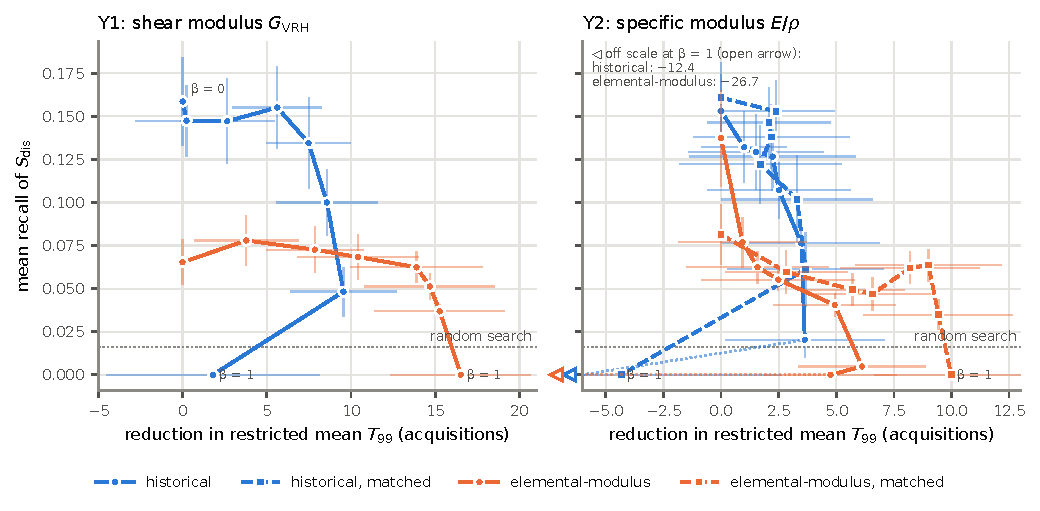
\includegraphics[width=\textwidth]{figures/fig1_frontier.pdf}
\caption{Efficiency--coverage frontier in the primary universe. Each point is one prior weight $\beta$ (from $\beta=0$ at zero
gain to $\beta=1$); bars are unadjusted two-sided 95\% split-level $t$ intervals (H1 tests the loss at $\beta=0.25$ and $0.5$,
and the H2 rule uses one-sided bounds at $\beta=0.02$--0.75; the bars themselves are descriptive). Horizontal axis: reduction in restricted mean sequential $\Tnn$ relative to $\beta=0$. Vertical axis: recall of $\Sdis$,
which is defined separately for each prior, so its level is compared within a curve only. The dotted line is the recall of
random search (Supplementary Table~\ref{S-tab:s-random}). Two $\beta=1$ points for Y2 lie off scale: their values are listed in
the panel, and they are drawn as open arrows outside the left edge of the axis with dotted leads, not to scale. All values are in Supplementary Table~\ref{S-tab:s-frontier}.}
\label{fig:frontier}
\end{figure*}

% ------------------------------------------------------------------------------
\subsection{Coverage loss at moderate prior weight differs between cells}\label{sec:h1}

\paragraph{What the coverage outcome measures.} $\Sdis$ is the half of the top-5\% materials that the cell's own prior scores
lowest. Its recall is therefore a prior-specific stress test: it asks whether weighting a prior costs the search the good
materials that this prior disfavours. It is not a measure of global coverage or diversity, and because the set is built from the
prior under test, some loss at high $\beta$ is built into it; Section~\ref{sec:where} adds the absolute blind spot $\Sblind$.
$L$ is an absolute difference in recall; where we give a loss relative to the baseline recall, we say so.

\paragraph{H1.} H1 asked whether a prior weight of 0.25 or 0.5 already reduces the recall of $\Sdis$, in 12 tests (two weights in each of six
cells) with Holm correction. A loss was detected in \R{h1cells/primary} of the 6 cells, at one or both weights, and
$H_0\colon L\le0$ was rejected in \R{h1count/primary} of the \R{h1n/primary} tests (Fig.~\ref{fig:h1}, Table~\ref{tab:h1h2}).
For the historical prior on Y2, in both its fixed and its matched form, and for the elemental-modulus prior on Y2, a loss was
detected at both weights; the largest was \cellE{} at $\beta=0.5$, $L=\R{h1/primary/Y2:P_phys_fixed/0.5/mean_L}$
\ci{h1/primary/Y2:P_phys_fixed/0.5/ci} in absolute recall, against a baseline recall of
\R{h2base/primary/Y2:P_phys_fixed/baseline_R_dis}: a relative loss of \R{h2detail/primary/Y2:P_phys_fixed/0.5/relative_loss}, nearly
all of the $\Sdis$ members that the no-prior search found. For the
historical prior on Y1, a loss was detected at $\beta=0.5$ ($L=\R{h1/primary/Y1:P_H_fixed/0.5/mean_L}$, Holm
$p$\R{h1/primary/Y1:P_H_fixed/0.5/p_holm_rel}) but not at 0.25 (Holm $p$\R{h1/primary/Y1:P_H_fixed/0.25/p_holm_rel}).

No loss was detected for the elemental-modulus prior on Y1 (Holm $p$\R{h1/primary/Y1:P_phys_fixed/0.25/p_holm_rel} at
$\beta=0.25$ and \R{h1/primary/Y1:P_phys_fixed/0.5/p_holm} at 0.5) or for its matched form on Y2 (Holm
$p$\R{h1/primary/Y2:P_phys_matched_Y2/0.25/p_holm_rel} and \R{h1/primary/Y2:P_phys_matched_Y2/0.5/p_holm}). For three of these four
tests the two-sided 95\% interval excludes zero; the intervals are unadjusted, whereas the tests are one-sided and
Holm-adjusted over 12 tests. A non-rejection means that no loss was detected, not that coverage was
preserved; whether a loss is demonstrably small is the question of H2 (Section~\ref{sec:h2}), and Section~\ref{sec:where} shows
that the absolute blind spot of the Y1 elemental-modulus prior is nevertheless lost at $\beta=0.5$.

\begin{figure}[t]
\centering
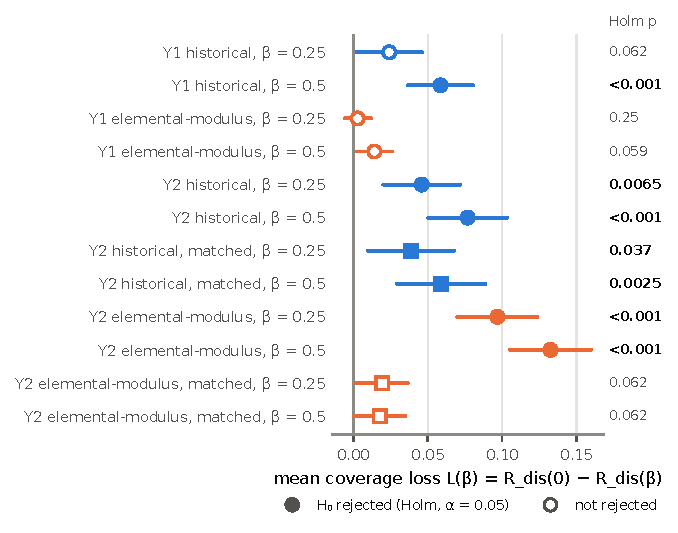
\includegraphics[width=\colw{0.72}]{figures/fig2_h1_forest.pdf}
\caption{H1: mean coverage loss $L(\beta)=\Rdis(0)-\Rdis(\beta)$ at $\beta=0.25$ and $0.5$ in the six primary cells, with
unadjusted two-sided 95\% split-level $t$ intervals. Filled markers: one-sided $H_0\colon L\le 0$ rejected after Holm correction over the 12 tests
($\alpha=0.05$); open markers: not rejected. Right: Holm-adjusted $p$.}
\label{fig:h1}
\end{figure}

% ------------------------------------------------------------------------------
\subsection{A beneficial weight that is safe under the registered criterion was found in three of six cells}\label{sec:h2}

H2 is a registered decision rule. A cell is applicable if the no-prior search finds members of $\Sdis$ above chance; all
\R{h2applicable/primary} cells were, with baseline recalls of \R{h2base/primary/Y1:P_phys_fixed/baseline_R_dis} to
\R{h2base/primary/Y2:P_H_matched_Y2/baseline_R_dis} against a chance recall of \R{h2base/primary/Y1:P_H_fixed/chance}. A weight
is \emph{beneficial} if the one-sided lower 95\% bound of the efficiency gain is above zero, and \emph{safe} if the upper bound,
at level $1-0.05/6$, of $L(\beta)-0.2\,\Rdis(0)$ is below zero, that is, if the search demonstrably loses less than 20\% of the
baseline's recall of $\Sdis$. Throughout, ``safe'' means safe under this criterion. The rule considers the six weights from
0.02 to 0.75. The safety level is adjusted across them, so that, if every weight truly loses 20\% or more, the statement ``at
least one weight is safe'' is wrong with probability at most 0.05 within a cell; the beneficial bound is not adjusted, and nothing
is adjusted across cells, whose decisions are not independent because the cells of an objective share their no-prior runs.

A beneficial and safe weight was found in \R{h2nonempty/primary} of the 6 cells (Fig.~\ref{fig:h2}, Table~\ref{tab:h1h2}):
\cellA{} \R{h2set/primary/Y1:P_H_fixed}, \cellB{} \R{h2set/primary/Y1:P_phys_fixed} and \cellD{}
\R{h2set/primary/Y2:P_H_matched_Y2}. None was found for \cellC{}, \cellE{} or \cellF{}, and no weight qualified in every cell.
Efficiency alone did not identify these weights: at $\beta=0.5$, \R{benefcount/primary/0.5} of the 6 cells were beneficial
and \R{safecount/primary/0.5} were safe. For \cellE{} the loss was large at every nonzero weight: at the smallest, $\beta=0.02$, it
already lost $L=\R{frontier/primary/Y2:P_phys_fixed/0.02/L}$ in absolute recall, a relative loss of
\R{h2detail/primary/Y2:P_phys_fixed/0.02/relative_loss} of the baseline, for a gain of \R{frontier/primary/Y2:P_phys_fixed/0.02/gain} \ci{frontier/primary/Y2:P_phys_fixed/0.02/gain}
acquisitions, and the relative loss rose with $\beta$ to \R{h2detail/primary/Y2:P_phys_fixed/0.75/relative_loss} at 0.75.

The 20\% margin is a judgement fixed before any result, and the sets depend on it. With a 10\% margin, a beneficial and safe
weight remained only for \cellB{} (\R{bs10/primary/Y1:P_phys_fixed}); with a 25\% margin the sets were \cellA{}
\R{bs25/primary/Y1:P_H_fixed}, \cellB{} \R{bs25/primary/Y1:P_phys_fixed} and \cellD{} \R{bs25/primary/Y2:P_H_matched_Y2}
(Table~\ref{tab:h1h2}). The registered rule does not control the error of the joint call: only its safety bound is adjusted across
the six weights. In a post hoc check (decision-log entry~44) with the beneficial bound also at level $1-0.05/6$, which bounds the
probability of any false beneficial-and-safe call in a cell by 0.10, a beneficial and safe weight remained in
\R{posthoc/h2adjnonempty/primary} of the 6 cells: \cellA{} \R{posthoc/bs20_adjusted/primary/Y1:P_H_fixed} and \cellB{}
\R{posthoc/bs20_adjusted/primary/Y1:P_phys_fixed}. The weight 0.02 dropped out of both \cellB{} (one-sided lower bound of the gain
\R{posthoc/h2adj/primary/Y1:P_phys_fixed/0.02/gain_lower95} at 95\%, \R{posthoc/h2adj/primary/Y1:P_phys_fixed/0.02/gain_lower_adjusted}
adjusted) and \cellD{} (\R{posthoc/h2adj/primary/Y2:P_H_matched_Y2/0.02/gain_lower95} and
\R{posthoc/h2adj/primary/Y2:P_H_matched_Y2/0.02/gain_lower_adjusted}), so the third cell's qualifying weight rests on the
unadjusted beneficial bound. The sets also depend on the curation of the benchmark. Without Pm and Tc (sensitivity universe~1), the
sets were \cellA{} \R{h2set/sens1_no_Pm_Tc/Y1:P_H_fixed}, \cellB{} \R{h2set/sens1_no_Pm_Tc/Y1:P_phys_fixed}, \cellC{}
\R{h2set/sens1_no_Pm_Tc/Y2:P_H_fixed} and \cellD{} \R{h2set/sens1_no_Pm_Tc/Y2:P_H_matched_Y2}, and none for the two Y2
elemental-modulus cells; without the reference screen (sensitivity universe~2, historical priors only), no cell had a beneficial
and safe weight (Supplementary Table~\ref{S-tab:s-universes}). The direction of H1 was the same in both sensitivity universes: every estimated loss at $\beta=0.25$ and $0.5$
was positive except \cellB{} at 0.25 without Pm and Tc ($L=\R{h1/sens1_no_Pm_Tc/Y1:P_phys_fixed/0.25/mean_L}$).

\begin{figure}[t]
\centering
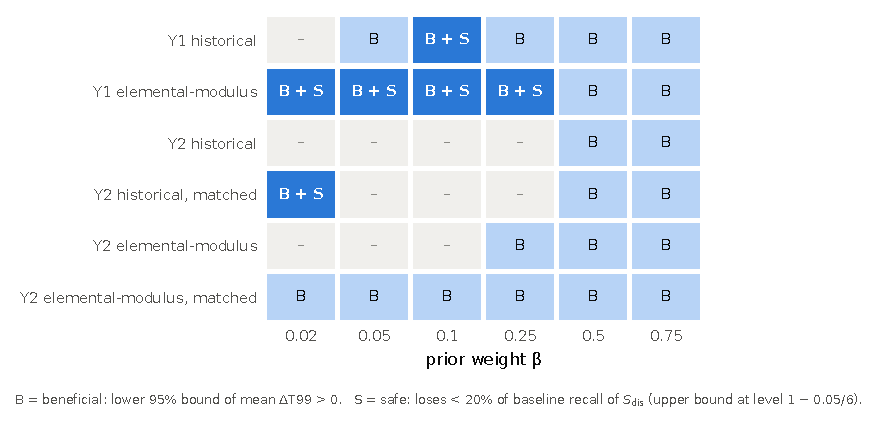
\includegraphics[width=\colw{0.78}]{figures/fig3_h2_grid.pdf}
\caption{H2 in the primary universe: for each cell and prior weight, whether the weight is beneficial (B), safe under the
registered criterion (S), both (B\,+\,S) or neither (--). The safety bound is at level $1-0.05/6$ within a cell.}
\label{fig:h2}
\end{figure}

\begin{table*}[t]
\centering\small
\caption{Main results in the primary universe. (a) Efficiency gain (reduction in restricted mean sequential $\Tnn$,
acquisitions) and coverage loss $L$ (absolute difference in recall of $\Sdis$), each with an unadjusted two-sided 95\%
split-level $t$ interval; $N_5$: mean number of top-5\% materials acquired in the 40 acquisitions (registered secondary;
\R{frontier/primary/Y1:P_H_fixed/0/N5} for Y1 and \R{frontier/primary/Y2:P_H_fixed/0/N5} for Y2 at $\beta=0$); $\Rdis(0)$: baseline
recall of $\Sdis$; $p_{\mathrm{H}}$: Holm-adjusted one-sided $p$ of H1 (12 tests).
(b) Weights that are beneficial and safe under the H2 rule with a safety margin of 10\%, 20\% (registered) and 25\%
(descriptive); last column: post hoc, with the beneficial bound also at level $1-0.05/6$. Cells: hist.\ = historical prior, elem.\ = elemental-modulus heuristic prior, m.\ = matched to Y2. H1 and H2 in full: Supplementary Tables~\ref{S-tab:s-h1} and~\ref{S-tab:s-h2}.}
\label{tab:h1h2}
\footnotesize\setlength{\tabcolsep}{3.5pt}
\textbf{(a)}\\[2pt]
\begin{tabular}{@{}lccccccccc@{}}
\toprule
 & & \multicolumn{4}{c}{$\beta=0.25$} & \multicolumn{4}{c}{$\beta=0.5$} \\
\cmidrule(lr){3-6}\cmidrule(l){7-10}
Cell & $\Rdis(0)$ & gain & $N_5$ & $L$ & $p_{\mathrm{H}}$ & gain & $N_5$ & $L$ & $p_{\mathrm{H}}$ \\
\midrule
\hrow{Y1 hist.}{Y1:P_H_fixed}
\hrow{Y1 elem.}{Y1:P_phys_fixed}
\hrow{Y2 hist.}{Y2:P_H_fixed}
\hrow{Y2 hist.\ m.}{Y2:P_H_matched_Y2}
\hrow{Y2 elem.}{Y2:P_phys_fixed}
\hrow{Y2 elem.\ m.}{Y2:P_phys_matched_Y2}
\bottomrule
\end{tabular}

\medskip
\textbf{(b)}\\[2pt]
\begin{tabular}{@{}lcccc@{}}
\toprule
 & \multicolumn{3}{c}{beneficial and safe $\beta$, safety margin} & \makecell{20\%, beneficial\\bound adjusted} \\
\cmidrule(lr){2-4}
Cell & 10\% & 20\% (registered) & 25\% & (post hoc) \\
\midrule
\srow{Y1 hist.}{Y1:P_H_fixed}
\srow{Y1 elem.}{Y1:P_phys_fixed}
\srow{Y2 hist.}{Y2:P_H_fixed}
\srow{Y2 hist.\ m.}{Y2:P_H_matched_Y2}
\srow{Y2 elem.}{Y2:P_phys_fixed}
\srow{Y2 elem.\ m.}{Y2:P_phys_matched_Y2}
\bottomrule
\end{tabular}
\end{table*}

% ------------------------------------------------------------------------------
\subsection{Robustness}\label{sec:robust}

\paragraph{Previously unanalysed splits.} Splits r0--r2 of each type were inspected during the exploratory phase; for the
other 14 (r3--r9) no discovery-side outcome had been computed before registration. On those 14 splits alone
(Table~\ref{tab:new}), the losses of the Y2 historical cells and of \cellE{} remained, for example
$L=\R{newsplits/primary/Y2:P_phys_fixed/0.5/L}$ \ci{newsplits/primary/Y2:P_phys_fixed/0.5/L} for \cellE{} at $\beta=0.5$, as did
the loss of \cellA{} at 0.5 ($L=\R{newsplits/primary/Y1:P_H_fixed/0.5/L}$ \ci{newsplits/primary/Y1:P_H_fixed/0.5/L}). \cellB{}
again combined a large gain, \R{newsplits/primary/Y1:P_phys_fixed/0.25/gain} \ci{newsplits/primary/Y1:P_phys_fixed/0.25/gain}
acquisitions at $\beta=0.25$, with no detected loss ($L=\R{newsplits/primary/Y1:P_phys_fixed/0.25/L}$). The gains of the Y2
historical cells were uncertain on these splits (\cellC{} at 0.5: \R{newsplits/primary/Y2:P_H_fixed/0.5/gain}
\ci{newsplits/primary/Y2:P_H_fixed/0.5/gain}). This is a robustness check within the same benchmark, not a replication: the
discovery pools of r3--r9 overlap 86--88\% with history sides that were used in engine tests and in the review before
registration, and the tests have at most 12 degrees of freedom.

\begin{table*}[t]
\centering\small
\caption{Previously unanalysed splits r3--r9 only (14 splits; descriptive). Gain: reduction in restricted mean $\Tnn$
(acquisitions); $L$: coverage loss; two-sided 95\% split-level $t$ intervals. All weights: Supplementary Table~\ref{S-tab:s-newsplits}.}
\label{tab:new}
\setlength{\tabcolsep}{5pt}
\begin{tabular}{@{}lcccc@{}}
\toprule
 & \multicolumn{2}{c}{$\beta=0.25$} & \multicolumn{2}{c}{$\beta=0.5$} \\
\cmidrule(lr){2-3}\cmidrule(l){4-5}
Cell & gain & $L$ & gain & $L$ \\
\midrule
\nrow{\cellA}{Y1:P_H_fixed}
\nrow{\cellB}{Y1:P_phys_fixed}
\nrow{\cellC}{Y2:P_H_fixed}
\nrow{\cellD}{Y2:P_H_matched_Y2}
\nrow{\cellE}{Y2:P_phys_fixed}
\nrow{\cellF}{Y2:P_phys_matched_Y2}
\bottomrule
\end{tabular}
\end{table*}

\paragraph{Budget.} Gains and losses appeared early in the campaign. Within the first 10 acquisitions, \cellB{} at
$\beta=0.25$ gained \R{budget/primary/Y1:P_phys_fixed/0.25/10/gain} acquisitions with
$L=\R{budget/primary/Y1:P_phys_fixed/0.25/10/L}$, while \cellE{} at $\beta=0.5$ lost $L=\R{budget/primary/Y2:P_phys_fixed/0.5/10/L}$
for a gain of \R{budget/primary/Y2:P_phys_fixed/0.5/10/gain} (Supplementary Table~\ref{S-tab:s-budget}; $\Tnn$ is restricted at $t+1$
for a budget of $t$ acquisitions).

\paragraph{Censoring and the initial design (post hoc).} Two checks were added after the registered analysis and are
exploratory. First, the share of runs without a top-1\% hit, for which $\Tnn=41$, was \R{posthoc/censor/primary/Y1:P_H_fixed/0}\%
(Y1) and \R{posthoc/censor/primary/Y2:P_H_fixed/0}\% (Y2) at $\beta=0$ and at most
\R{posthoc/censor/primary/Y2:P_H_matched_Y2/0.25}\% at $\beta=0.25$--0.75 in any cell (Supplementary Table~\ref{S-tab:s-censor}).
Second, the shared initial design already contained a top-1\% material in \R{posthoc/inittop1/primary/Y1} (Y1) and
\R{posthoc/inittop1/primary/Y2} (Y2) of \R{posthoc/initblocks/primary/Y1} split--seed blocks (Supplementary Table~\ref{S-tab:s-init}); scoring those blocks as discovered
at time zero changed the primary gains at $\beta\le0.75$ by at most \R{posthoc/initsens/maxshift/primary} acquisitions. It turned
\R{posthoc/initsens/nflips/primary} weight beneficial (\cellC{} at $\beta=0.25$), which is not safe, and changed no beneficial and
safe set.

\paragraph{Split type (post hoc).} Estimated within each split type separately (decision-log entry~45; 10 splits each, descriptive),
\R{posthoc/splittype/signagree/primary} of the \R{posthoc/splittype/n/primary} point estimates of gain and loss at $\beta=0.25$
and $0.5$ had the same sign as the registered estimate (Supplementary Table~\ref{S-tab:s-splittype}). Because the registered
estimate is the mean of the two, at least one of each pair must agree, and \R{posthoc/splittype/includezero/primary} of the
\R{posthoc/splittype/n/primary} intervals include zero. Their sizes could differ: the loss of \cellA{} at $\beta=0.25$ was $L=\R{posthoc/splittype/primary/Y1:P_H_fixed/0.25/L/random/estimate}$
[\R{posthoc/splittype/primary/Y1:P_H_fixed/0.25/L/random/ci_lo}, \R{posthoc/splittype/primary/Y1:P_H_fixed/0.25/L/random/ci_hi}]
on the random splits and \R{posthoc/splittype/primary/Y1:P_H_fixed/0.25/L/chemsys/estimate}
[\R{posthoc/splittype/primary/Y1:P_H_fixed/0.25/L/chemsys/ci_lo}, \R{posthoc/splittype/primary/Y1:P_H_fixed/0.25/L/chemsys/ci_hi}]
on the chemical-system splits, although the two intervals overlap. Over all weights, \R{posthoc/splittype/opposite/primary} of the
\R{posthoc/splittype/n_all/primary} split-type intervals lay entirely on the other side of zero from the registered estimate,
with no adjustment for their number. It concerns the prior-only search ($\beta=1$) of \cellD{}, whose registered gain was
\R{frontier/primary/Y2:P_H_matched_Y2/1/gain}: on the random splits the gain was
\R{posthoc/splittype/primary/Y2:P_H_matched_Y2/1/gain/random/estimate}
[\R{posthoc/splittype/primary/Y2:P_H_matched_Y2/1/gain/random/ci_lo}, \R{posthoc/splittype/primary/Y2:P_H_matched_Y2/1/gain/random/ci_hi}]
acquisitions, above zero, and on the chemical-system splits \R{posthoc/splittype/primary/Y2:P_H_matched_Y2/1/gain/chemsys/estimate}
[\R{posthoc/splittype/primary/Y2:P_H_matched_Y2/1/gain/chemsys/ci_lo}, \R{posthoc/splittype/primary/Y2:P_H_matched_Y2/1/gain/chemsys/ci_hi}].

% ------------------------------------------------------------------------------
\subsection{Where the guided searches find their materials}\label{sec:where}

Weighting the prior changed how many top-5\% materials the search acquired as well as which. Without a prior the search
acquired on average $N_5=\R{frontier/primary/Y1:P_H_fixed/0/N5}$ \ci{frontier/primary/Y1:P_H_fixed/0/N5} of them in 40
acquisitions for Y1 and \R{frontier/primary/Y2:P_H_fixed/0/N5} \ci{frontier/primary/Y2:P_H_fixed/0/N5} for Y2. At $\beta=0.5$,
$N_5$ was higher than without a prior in \R{n5up/primary/0.5} of the 6 cells, for example
\R{frontier/primary/Y1:P_phys_fixed/0.5/N5} \ci{frontier/primary/Y1:P_phys_fixed/0.5/N5} for \cellB{} and
\R{frontier/primary/Y2:P_H_matched_Y2/0.5/N5} \ci{frontier/primary/Y2:P_H_matched_Y2/0.5/N5} for \cellD{}, while their
estimated recall of $\Sdis$ was lower, a loss detected by H1 in \R{n5up_h1/primary/0.5} of them (Table~\ref{tab:h1h2}). In those
cells the weighted search found more good materials in total but, by its point estimates, fewer of those its prior disfavours,
consistent with the shift of its discoveries toward the prior's top-ranked materials (Fig.~\ref{fig:bins}): it redirected the
search rather than reducing what it found. \cellE{} is the exception: its $N_5$ was \R{frontier/primary/Y2:P_phys_fixed/0.5/N5}
\ci{frontier/primary/Y2:P_phys_fixed/0.5/N5}, so it lost coverage without finding more good materials. $N_5$ is a registered
secondary outcome; these comparisons are descriptive, and its intervals are for its level, not for the difference from $\beta=0$.

As $\beta$ grew, the top-5\% materials found by the search shifted toward the materials the prior ranks highest
(Fig.~\ref{fig:bins}). At $\beta=1$, no top-5\% material below the prior's 95th percentile was found in any cell; at $\beta=0$
the search found, for example, a fraction \R{rbins/primary/Y2:P_H_fixed/0/0.0/recall} of the \cellC{} top-5\% materials in the
prior's lowest half. This describes where the guided search goes; it is not by itself a demonstration of the cause of the
trade-off.

The same shift appears in the absolute blind spot $\Sblind$, the top-5\% materials below the prior's 80th percentile. In a post
hoc analysis (decision-log entry~43) with the registered split-level estimator, the loss of its recall,
$L_{\mathrm{blind}}(\beta)=R_{\mathrm{blind}}(0)-R_{\mathrm{blind}}(\beta)$, had a 95\% interval above zero in
\R{posthoc/blindcount/primary/0.5} of 6 cells at $\beta=0.5$ and in \R{posthoc/blindcount/primary/0.25} of 6 at $\beta=0.25$
(Supplementary Table~\ref{S-tab:s-blind}). The exception at 0.25 is \cellB{}: $L_{\mathrm{blind}}=\R{posthoc/blind/primary/Y1:P_phys_fixed/0.25/L_blind}$
\ci{posthoc/blind/primary/Y1:P_phys_fixed/0.25/L_blind} at $\beta=0.25$, but \R{posthoc/blind/primary/Y1:P_phys_fixed/0.5/L_blind}
\ci{posthoc/blind/primary/Y1:P_phys_fixed/0.5/L_blind} at 0.5, against a baseline recall of
\R{posthoc/blind/primary/Y1:P_phys_fixed/0/R_blind}, so almost all of this prior's blind spot was lost at $\beta=0.5$. This coexists
with no detected loss of $\Sdis$ at $\beta=0.5$ (Section~\ref{sec:h1}): that prior ranks most of its top-5\% materials highly, so
its $\Sblind$ is small (\R{frontier/primary/Y1:P_phys_fixed/0/S_blind_mean_size} materials per run on average) and most of its
$\Sdis$ (62--64 materials) lies above its 80th percentile. Because $\Sdis$ is selected on low prior score, some loss at high
$\beta$ is built into its definition; $\Sblind$ is the less constructed measure.

Two checks indicate that the searches behaved as designed. With the prior reversed at $\beta=0.5$, the search was slower than
without a prior in every cell: the gain was between \R{manip/primary/Y2:P_H_fixed/0.5/gain_P_wrong} (\cellC{}) and
\R{manip/primary/Y2:P_phys_matched_Y2/0.5/gain_P_wrong} (\cellF{}) acquisitions, with every interval below zero. In no step of any
arm did the group of candidates tied at the highest EI hold more than half of the candidates, and the GP length-scale was at its lower bound in
\R{healthrange/primary/lb_min}--\R{healthrange/primary/lb_max}\% of steps per arm (Supplementary Table~\ref{S-tab:s-health}). A registered candidate-level mixed model agrees with the shift in direction at
$\beta\ge0.25$ only; it is reported in Supplementary Note~\ref{S-note:glmm} and Supplementary Table~\ref{S-tab:s-glmm}, where its limitations (near-separation;
\R{summary/glmm_nonconverged} of 6 fits not converged) are discussed, and we do not interpret its effect sizes.

\begin{figure*}[t]
\centering
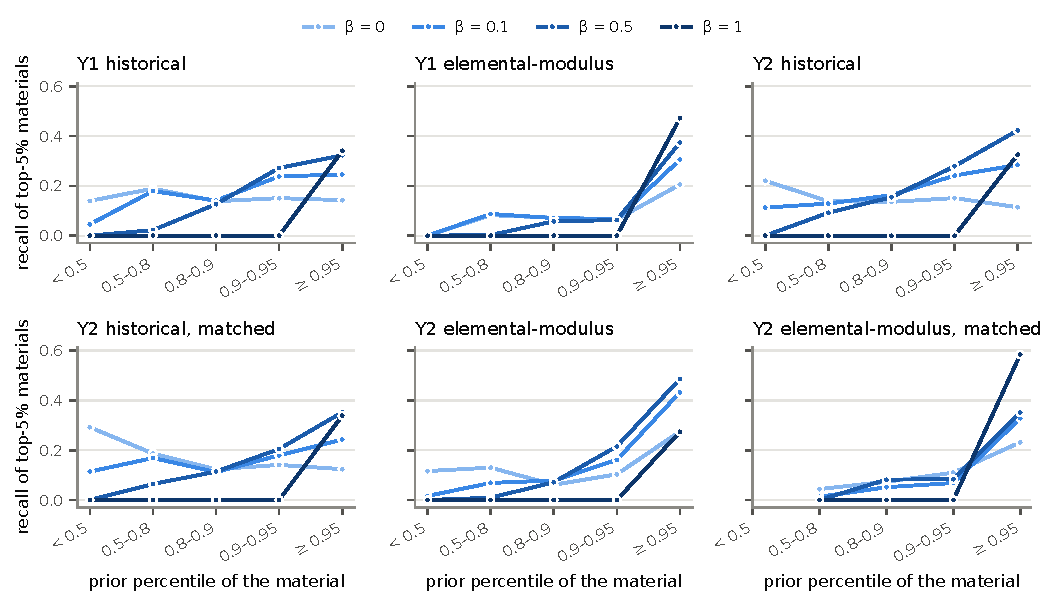
\includegraphics[width=\textwidth]{figures/fig4_recall_bins.pdf}
\caption{Recall of top-5\% materials by prior-percentile bin, pooled over the 60 runs of each arm, at four prior weights
(primary universe). Some bins are small (for \cellB{} the lowest bin holds
\R{rbins/primary/Y1:P_phys_fixed/0/0.0/available} material--runs in total; for \cellF{} it is empty).}
\label{fig:bins}
\end{figure*}

% ------------------------------------------------------------------------------
\subsection{The prior-only boundary case and pre-search alignment}\label{sec:bound}

At $\beta=1$ the search ranks candidates by the prior alone; it is a reference point, not Bayesian optimisation with a strong
prior. For the two fixed priors on Y2 it was much slower than the no-prior search, with gains of \R{frontier/primary/Y2:P_H_fixed/1/gain}
\ci{frontier/primary/Y2:P_H_fixed/1/gain} (\cellC{}) and \R{frontier/primary/Y2:P_phys_fixed/1/gain}
\ci{frontier/primary/Y2:P_phys_fixed/1/gain} (\cellE{}) acquisitions; it found no top-1\% material in
\R{posthoc/censor/primary/Y2:P_H_fixed/1}\% and \R{posthoc/censor/primary/Y2:P_phys_fixed/1}\% of these runs (post hoc,
Section~\ref{sec:robust}), so the restricted mean probably understates the slowdown. For \cellB{} and \cellF{} it was faster, by
\R{frontier/primary/Y1:P_phys_fixed/1/gain} \ci{frontier/primary/Y1:P_phys_fixed/1/gain} and
\R{frontier/primary/Y2:P_phys_matched_Y2/1/gain} \ci{frontier/primary/Y2:P_phys_matched_Y2/1/gain} acquisitions; for \cellA{}
(\R{frontier/primary/Y1:P_H_fixed/1/gain} \ci{frontier/primary/Y1:P_H_fixed/1/gain}) and \cellD{}
(\R{frontier/primary/Y2:P_H_matched_Y2/1/gain} \ci{frontier/primary/Y2:P_H_matched_Y2/1/gain}) the interval includes zero.

Across the six cells, the history-side rank correlation between prior and objective and the gain at $\beta=0.5$ went together
(Kendall $\tau=\R{summary/tau}$, $n=6$; exploratory H3, registered without a test). With six cells, a $\tau$ this large is
compatible with no association (exact two-sided $p=\R{summary/tau_p_exact}$, computed for orientation only). The six cells share objectives, prior constructions and the pool, so this is
a hypothesis for future work, not evidence that alignment determines the frontier.

\subsection{Summary}\label{sec:summary}
Across the six prior--objective cells, the effects of weighting a prior differed. The elemental-modulus heuristic prior reduced
the restricted mean sequential $\Tnn$ for Y1 by \R{frontier/primary/Y1:P_phys_fixed/0.25/gain}
\ci{frontier/primary/Y1:P_phys_fixed/0.25/gain} acquisitions at $\beta=0.25$ with no detected loss of $\Sdis$ and, at that weight,
no detected loss of its blind spot (post hoc); at $\beta=0.5$ it lost almost all of the blind spot. For Y2, the fixed form of the
same prior lost a large share of $\Sdis$ at every nonzero weight, from the smallest. A weight that is beneficial and safe under the
registered criterion was found in three of six cells, two of six when the beneficial bound is also adjusted (post hoc), and the
sets changed with the safety margin and with the curation of the benchmark. These results do not establish a universal efficiency--coverage relationship or a generally best prior weight. They
show that efficiency gains alone do not establish that a prior-weighted search keeps the good materials its prior disfavours.

